\documentclass{amsart}

\input{../preamble_general.tex}

\author{Jalen Chrysos}
\title{Random Walks \& Another Proof of Cayley's Formula (with Solutions)}

\begin{document}
	\maketitle 
	
	Given a graph $G$, a \textit{random walk} on $G$ is a sequence of vertices $V_0,V_1,\dots$ in which each $V_{j+1}$ is chosen uniformly from among the neighbors of $V_{j}$.\\
	
	\begin{minipage}{0.6\textwidth}
		\noindent \textbf{Problem 1}: In the graph shown, a random walk $w$ begins at $X$ and will end upon reaching $A$.\\
		\begin{enumerate}[(a)]
			\item What is the probability that $w$ visits $C$?
			\item What is the probability that $w$ visits $B$?
			\item What is the probability that $w$ visits $B$, $C$, and $D$?
		\end{enumerate}
	\end{minipage}
	\hspace{0.7cm}
	\begin{minipage}{0.5\textwidth}
		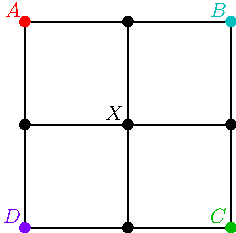
\includegraphics[width=0.5\textwidth]{./Asymptote_Figs/walk1.pdf}
	\end{minipage}
	
	\textbf{Solution}: \\
	
	(a): Walks visiting $C$ before $A$ and walks visiting $A$ before $C$ are equally likely: rotating by 180 degrees is a map between them which does not affect their probability. Thus the probability of visiting $C$ is 1/2.\\
	
	(b): Similarly, walks visiting $B$ before $A$ are reflected across a vertical line from walks visiting $A$ before $B$. Thus the probability of visiting $B$ is also 1/2.\\
	
	(c): Every walk visits one of $A,B,C,D$ last. Rotation 90 degrees changes which of these is the last to be visited, so the probability of visiting $B,C,D$, or equivalently visiting $A$ last, is 1/4.\\
	
	\noindent Given a walk $w$, the \textit{\textbf{loop-erasure}} of $w$, denoted $w'$, is a \textit{path} with edges from $w$, formed by always taking the last edge (in the order of $w$) leaving the current vertex:
	$$ (a,b,c,d,a,d,a,b,c,\underline{a,e},d,c,\underline{e,d},c,\underline{d,b},c,\underline{b,f}) \; \; \; \mapsto \;\;\; 
	(a,e,d,b,f)
	$$
	%	
	%	$$\textbf{diagram of loop-erasure}$$
	
	\noindent \textit{\textbf{Wilson's Algorithm}} is a method of randomly generating a spanning tree of $G$. Let the vertex-set of $G$ be $\{0,1,2,\dots,n-1\}$.
	\begin{enumerate}[(1)]
		\item Initially set $T = \{0\}$.
		\item Letting $X$ be the least vertex of $G$ not in $T$, produce a random walk $w$ that begins at $X$ and ends when it first hits a vertex of $T$.
		\item Expand $T$ by adding the vertices and edges of $w'$, the loop-erasure of $w$.
		\item If $T$ is not a spanning tree yet, return to step (2); otherwise, output $T$.\\
	\end{enumerate}
		\begin{figure}[h]
				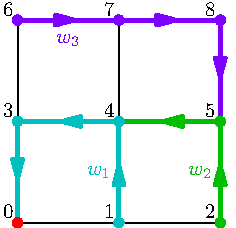
\includegraphics[width=4cm]{./Asymptote_Figs/Wilson.pdf}
			\end{figure}
		\textbf{Fact}: Every spanning tree of $G$ is equally likely to be the output of Wilson's algorithm\footnote{I will omit the proof of this, but if you want to see one you can read section 4.1 of \href{https://rdlyons.pages.iu.edu/prbtree/book_pb.pdf}{Probability on Trees and Networks} by Lyons and Peres.}. This is not such an easy thing to prove, but it becomes much easier when $G=K_n$.\\
	
	\noindent \textbf{Problem 2}: Now we will prove the correctness of Wilson's Algorithm in the case $G=K_n$ by taking an arbitrary spanning tree $T$ of $K_n$ and showing that the probability that Wilson's Algorithm produces this tree is exactly $1/n^{n-2}$. This constitutes another proof of Cayley's Formula.
	
	\textit{In this problem, to simplify some calculations, you can assume that every vertex has an edge to itself, so that from any vertex, there is exactly a $1/n$ chance of moving to any vertex, including $v$. This does not affect the probability that Wilson's algorithm outputs $T$ (check).}
	
	\begin{enumerate}[(a)]
		\item Show that $T$ can be the output of Wilson's Algorithm.
		\item Show that there is \textit{exactly one} sequence of paths $w'_1,w'_2,\dots,w'_k$ which results in the tree $T$.
		\item Find the probability that the first walk $w_1$ is exactly $w'_1$ (the length of $w'_1$ matters)
		\item Find the probability that $w_1$ consists of a single loop at $1$ (not visiting $0$) followed by $w'_1$. 
		\item Find the probability that $w_1$ consists of some number $k\geq 0$ of loops at 1, followed by $w'_1$.
		\item Find the probability that the first path produced by the algorithm is $w_1'$.
		\item Finally find the probability that the algorithm produces exactly the desired sequence of paths $w'_1,w'_2,\dots,w'_k$, i.e. the probability that the resulting tree is $T$.\\
	\end{enumerate}
	
	
	\textbf{Solution}: \\
	
	(a)+(b): At every stage of the construction, any vertex $v$ has a unique path in $T$ that takes it to 0 (because $T$ is a tree), so when we add a path from $v$ it must be this one.\\
	
	(c): For each vertex of the path $w'_1$, there is a $1/n$ probability of traveling to the correct next vertex, so the probability is $(1/n)^{|w'_1|}$ where $|w'_1|$ is the number of edges of $w'_1$.\\
	
	(d): The probability of $w_1$ hitting its starting vertex $1$ before $0$ is $1/2$ by symmetry; every vertex is adjacent to both $0$ and $1$ because $G=K_n$. Thus the probability is $(1/2)\cdot (1/n)^{|w'_1|}$.\\
	
	(e): The probability of looping once is $1/2$, the probability of looping twice is $1/4$, etc, so the probability of looping some number of times (including 0) is $1 + 1/2+1/4+\cdots = 2$. Thus the probability of some number of loops followed by $w'_1$ is $2\cdot (1/n)^{|w'_1|}$.\\
	
	(f): In addition to looping some number of times at 1, $w_1$ may loop some number of times at each vertex of $w'_1$. Let $v_j$ be the $j$th vertex of the path. The probability of a loop at $v_j$ is the same as the probability of hitting $v_j$ before hitting any of the $j-1$ previous vertices or vertex 0, which (by symmetry) is $(1/j)$. The probability of some number of loops at $v_j$ (including 0) is thus 
	$$1 + (1/j) + (1/j)^2 + \cdots = \frac{j+1}{j}.$$
	The probability of producing the loop-erased walk $w'_1$ is therefore 
	$$
	\Big(\frac{1}{n}\Big)^{|w'_1|} \cdot \big(2\big) \bigg(\frac{3}{2} \bigg)\bigg( \frac{4}{3}\bigg)\cdots \bigg(\frac{|w'_1| + 1}{|w'_1|}\bigg) = \Big(\frac{1}{n}\Big)^{|w'_1|} \cdot \bigg(\frac{|w'_1|+1}{1}\bigg).
	$$
	
	(g): Similarly to (f), the probability of producing the loop-erased walk $w'_2$ is 
	$$
	\Big(\frac{1}{n}\Big)^{|w'_2|} \cdot \bigg(\frac{|w'_1|+2}{|w'_1|+1}\bigg) \cdots\bigg( \frac{|w'_1|+|w'_2|+1}{|w'_1|+|w'_2|}\bigg) = \Big(\frac{1}{n}\Big)^{|w'_2|} \bigg(\frac{|w'_1|+|w'_2|+1}{|w'_1|+1}\bigg)
	$$
	and so on, yielding a total probability of
	\begin{align*}
	&= \Big(\frac{1}{n}\Big)^{|w'_1|}\Big(\frac{1}{n}\Big)^{|w'_2|} \cdots \Big(\frac{1}{n}\Big)^{|w'_k|} \cdot \bigg(\frac{|w'_1|+1}{|w'_1|}\bigg)   \bigg(\frac{|w'_1|+|w'_2|+1}{|w'_1|+1}\bigg) \cdots \bigg(\frac{|w'_1| + |w'_2| + \cdots + |w'_k|+1}{|w'_1| + |w'_2| + \cdots + |w'_{k-1}| + 1}\bigg) \\
	&= \Big(\frac{1}{n}\Big)^{|w'_1|+\cdots+|w'_k|} \cdot \Big(|w'_1| + \cdots + |w'_k| + 1\Big)\\
	&= \Big(\frac{1}{n}\Big)^{n-1} \cdot n\\
	&= \frac{1}{n^{n-2}}
	\end{align*}
	as expected.
\end{document}